\documentclass[10pt]{scrartcl}
\setlength{\textwidth}{16cm}
\setlength{\textheight}{26cm}
\setlength{\evensidemargin}{0cm}
\setlength{\oddsidemargin}{0cm}
\setlength{\topmargin}{-1cm}
\usepackage[english]{babel}
\usepackage[utf8]{inputenc}
\usepackage{amssymb,amsmath}
\usepackage[table,xcdraw]{xcolor}
\usepackage{array}
\usepackage{soul}
\usepackage{color}
\usepackage{subcaption}
\usepackage[shortlabels]{enumitem}
\usepackage{textcomp}
\usepackage{wasysym}
\usepackage{graphicx}
\usepackage{hyperref}


\setlist[itemize]{label=--}

\newcommand{\vsp}{\vspace*{1cm}}


\newcommand\tr{\ensuremath{\mathbf{t}}}
\newcommand\f{\ensuremath{\mathbf{f}}}
\newcommand\E{\exists}
\newcommand\A{\forall}
\newcommand\limplies{\supset}
%\def\lfi{\limplies}
\newcommand{\ABg}{\ensuremath{AB^=}}  %
\newcommand{\Sg}{{\ensuremath{S^=\colon}}}
\newcommand\INT{{\cal I}}



\begin{document}


\begin{center}{\LARGE\bfseries\sffamily
Self Organizing Systems 2022W\\
Assignment 1: Christmas market with GA}\\
Group 12: \\
Gawor Adrian Jan 11905152\\
Braunsperger Martin 11909911\\
Blohm Peter 11905150\\
\end{center}
\medskip

\sloppy


\section{Problem Description}

The Time-constrained "Travelling Christmas market visitor" problem is one of the custom problems described in the given PDF.

As a quick summary:

Given the locations and opening times of various Christmas markets all around Vienna, one wants to find a route to visit as many of them in a single day as possible.

\begin{itemize}
	\item Each market may only be visited at most once and only during open hours.
	\item The time spent at a market is exactly 30 minutes.
	\item Travelling time between markets must be accounted for.
\end{itemize}


\section{Representation of the Problem Domain}

While explicitly stated in the problem description, that this problem is not technically a version of the TSP, we still chose to represent the solution as such, a permutation which dictates the order in which the markets are visited. 

This encodes some properties of the problem quite nicely, and using a different target function, all constraints can be expressed.

One disadvantage this approach could cause is that changes to later parts of a solution will not affect the fitness, since markets later in the list will not be visited at all, regardless of their relative order.

Changes to these parts of the solution, however, could be viewed as silent mutations, and higher mutation rates will counteract these non-visible changes.

Before solving the actual problem, however, some amount of preprocessing is needed to get a usable instance akin to TSP.
% Special Case of TSP -> solved with GA implementation for TSP (preselection of operators)

\subsection{Preprocessing}

Since the location of the markets was only given as links to their Google-Maps entry, the preprocessing was performed in two steps.

First, the coordinates of the markets were obtained.
This was done by sending requests to Google for those resources.
Since, depending on the link, either the page or the URL of the entry will contain the latitude and longitude of the location, they can be grabbed from the responses via regex.

Afterwards, using the Matrix-API of \href{https://openrouteservice.org/}{Openroute Service}, which uses the OSRM, was used to get a matrix of \emph{walking} durations between all locations.

The reason the walking durations were used was that there were no free API's for public transport in Vienna found and driving after a few Glühweins could impact the travel times significantly.

To gauge performance of the algorithm depending on the instance size, a few other instances were generated from random locations around Vienna, but using the real walking times between those.
Since the time-constraint limits the quality of the solution, these instances use closing times \emph{after 24:00}, which is of course unreasonable but causes no problems in the chosen implementation.

Alternatively, walking and staying durations could be shortened until satisfactorily large solutions are possible.

\subsection{Target Function}

As mentioned above, the problem was essentially encoded as a TSP variation with following target function:
Starting at the first opening time of an instance, the walking times throughout the day are accumulated, keeping the time of arrival for each market in mind.

If a market is visited before it is opened, the person is assumed to \emph{wait until it is open} and only then continue the journey.

When a market is visited that closes either before the arrival or during the stay, the journey is over.

Since the total time frame as well as the duration of stay per market is fixed, minimizing the walking times then has the same effect as maximising the time spend on markets which is the same as maximising the amount of visited markets.

An interesting question to ask is whether to count markets which close during the stay and are not visited for the full 30 minutes.

While this does not influence the actual target function, we decided to include closing markets into the solution, which is important when looking at the resulting numbers for the visited markets.

\section{GA implementation}

Our approach to solve this problem was using genetic algorithms.
An existing implementation for genetic algorithms was used from the \href{https://scikit-optimize.github.io/stable/}{scikit-optimize} library, which had a specific preset for the TSP.

This preset is defined by the default set of operators which will be described below:

\begin{itemize}
    \item Mutate-Reverse aka 2-Opt

    A random section of the solution will be reversed, which for the conventional TSP corresponds to a 2-Opt-like mutation.
    \item Tournament selection with groups of 3
    Based on the ranking by the target function as described above.
    \item PMX-Crossover
    
    This modified version of crossover was already described in the lecture as an adaptation for TSP and starts by copying a chunk of one parent solution and filling the other values in a way as to still produce a valid permutation.
\end{itemize}
% TODO
% While there are many different hyper-parameters to tune, tried playin

\section{Results}

To analyse the behaviour of the chosen approach, results were collected for different population sizes and different iteration limits. 
It is to note that for each iteration limit, the algorithm as completely restarted, and did not just continue from a previously measured state.

The results were according to expectations: population size as well as iteration limits increased the individual run-time by a linear factor respectively.

A resulting plot for this experiment can be seen in figure \ref{fig:default_results}, clearly showing the linear increases of runtime but on the contrary a slight average increase of the visited markets.
An example of a found route is shown via a screenshot of google maps in figure \ref{fig:optimal_route}.

Plots of different instances, also included in the submission, showed that the amount of iterations until good solutions are found, also as expected, increases very fast with the amount of possible stops.

Choosing stopping criteria by amounts of iterations without improvement seems to be a good idea as in most cases more or less linear improvement can be seen until a sudden stop.


As a second experiment, the different settings for the selection operator in figure \ref{fig:selection} and for the mutation operator in figure \ref{fig:mutation} are shown.
The defaults proved to be fine, but another mutation operator, the swap-mutation, where two different stops are, as implied, swapped, seems to produce more consistent results.

% Explain experiment setup, the effect of population size and iterations, interpret plots etc.

% Maybe interesting to point out that population size was a linear factor, meaning the choice of the optimal population size is not that obvious.
% Larger populations showed good results seemingly a bit more reliable. 

% TODO: Route here?


% 1. 09:00 - Mittelalterlicher Adventmarkt
% 	Walking 13 minutes and 5 seconds
% 2. 10:00 - Belvedere
% 	Walking 29 minutes
% 3. 11:00 - Stephansplatz
% 	Walking 5 minutes and 57 seconds
% 4. 11:35 - Opera
% 	Walking 7 minutes and 32 seconds
% 5. 12:13 - Advent in der Stallburg
% 	Walking 7 minutes
% 6. 12:50 - Am Hof
% 	Walking 2 minutes and 20 seconds
% 7. 13:22 - Biobauern-Adventmarkt
% 	Walking 0 seconds
% 8. 13:52 - Altwiener Christkindlmarkt
% 	Walking 5 minutes and 20 seconds
% 9. 14:28 - Weihnachtsmarkt am Michaelerplatz
% 	Walking 16 minutes and 56 seconds
% 10. 15:15 - Karlsplatz
% 	Walking 20 minutes and 30 seconds
% 11. 16:05 - Spittelberg
% 	Walking 14 minutes and 22 seconds
% 12. 16:49 - Rathaus
% 	Walking 9 minutes and 36 seconds
% 13. 17:29 - Maria-Theresien-Platz
% 	Walking 16 minutes and 7 seconds
% 14. 18:15 - Adventmarkt Mariahilf
% 	Walking 15 minutes and 11 seconds
% 15. 19:00 - IKEA Westbahnhof
% 	Walking 21 minutes and 53 seconds
% 16. 19:52 - Messe
% 	Walking 22 minutes and 57 seconds
% 17. 20:45 - Ottakringer Weihnachtszauber
% 	Walking 25 minutes and 26 seconds
% 18. 21:41 - Altes AKH
% 	Walking 22 minutes and 10 seconds
% 19. 22:33 - MQ

\begin{figure}
    \centering
    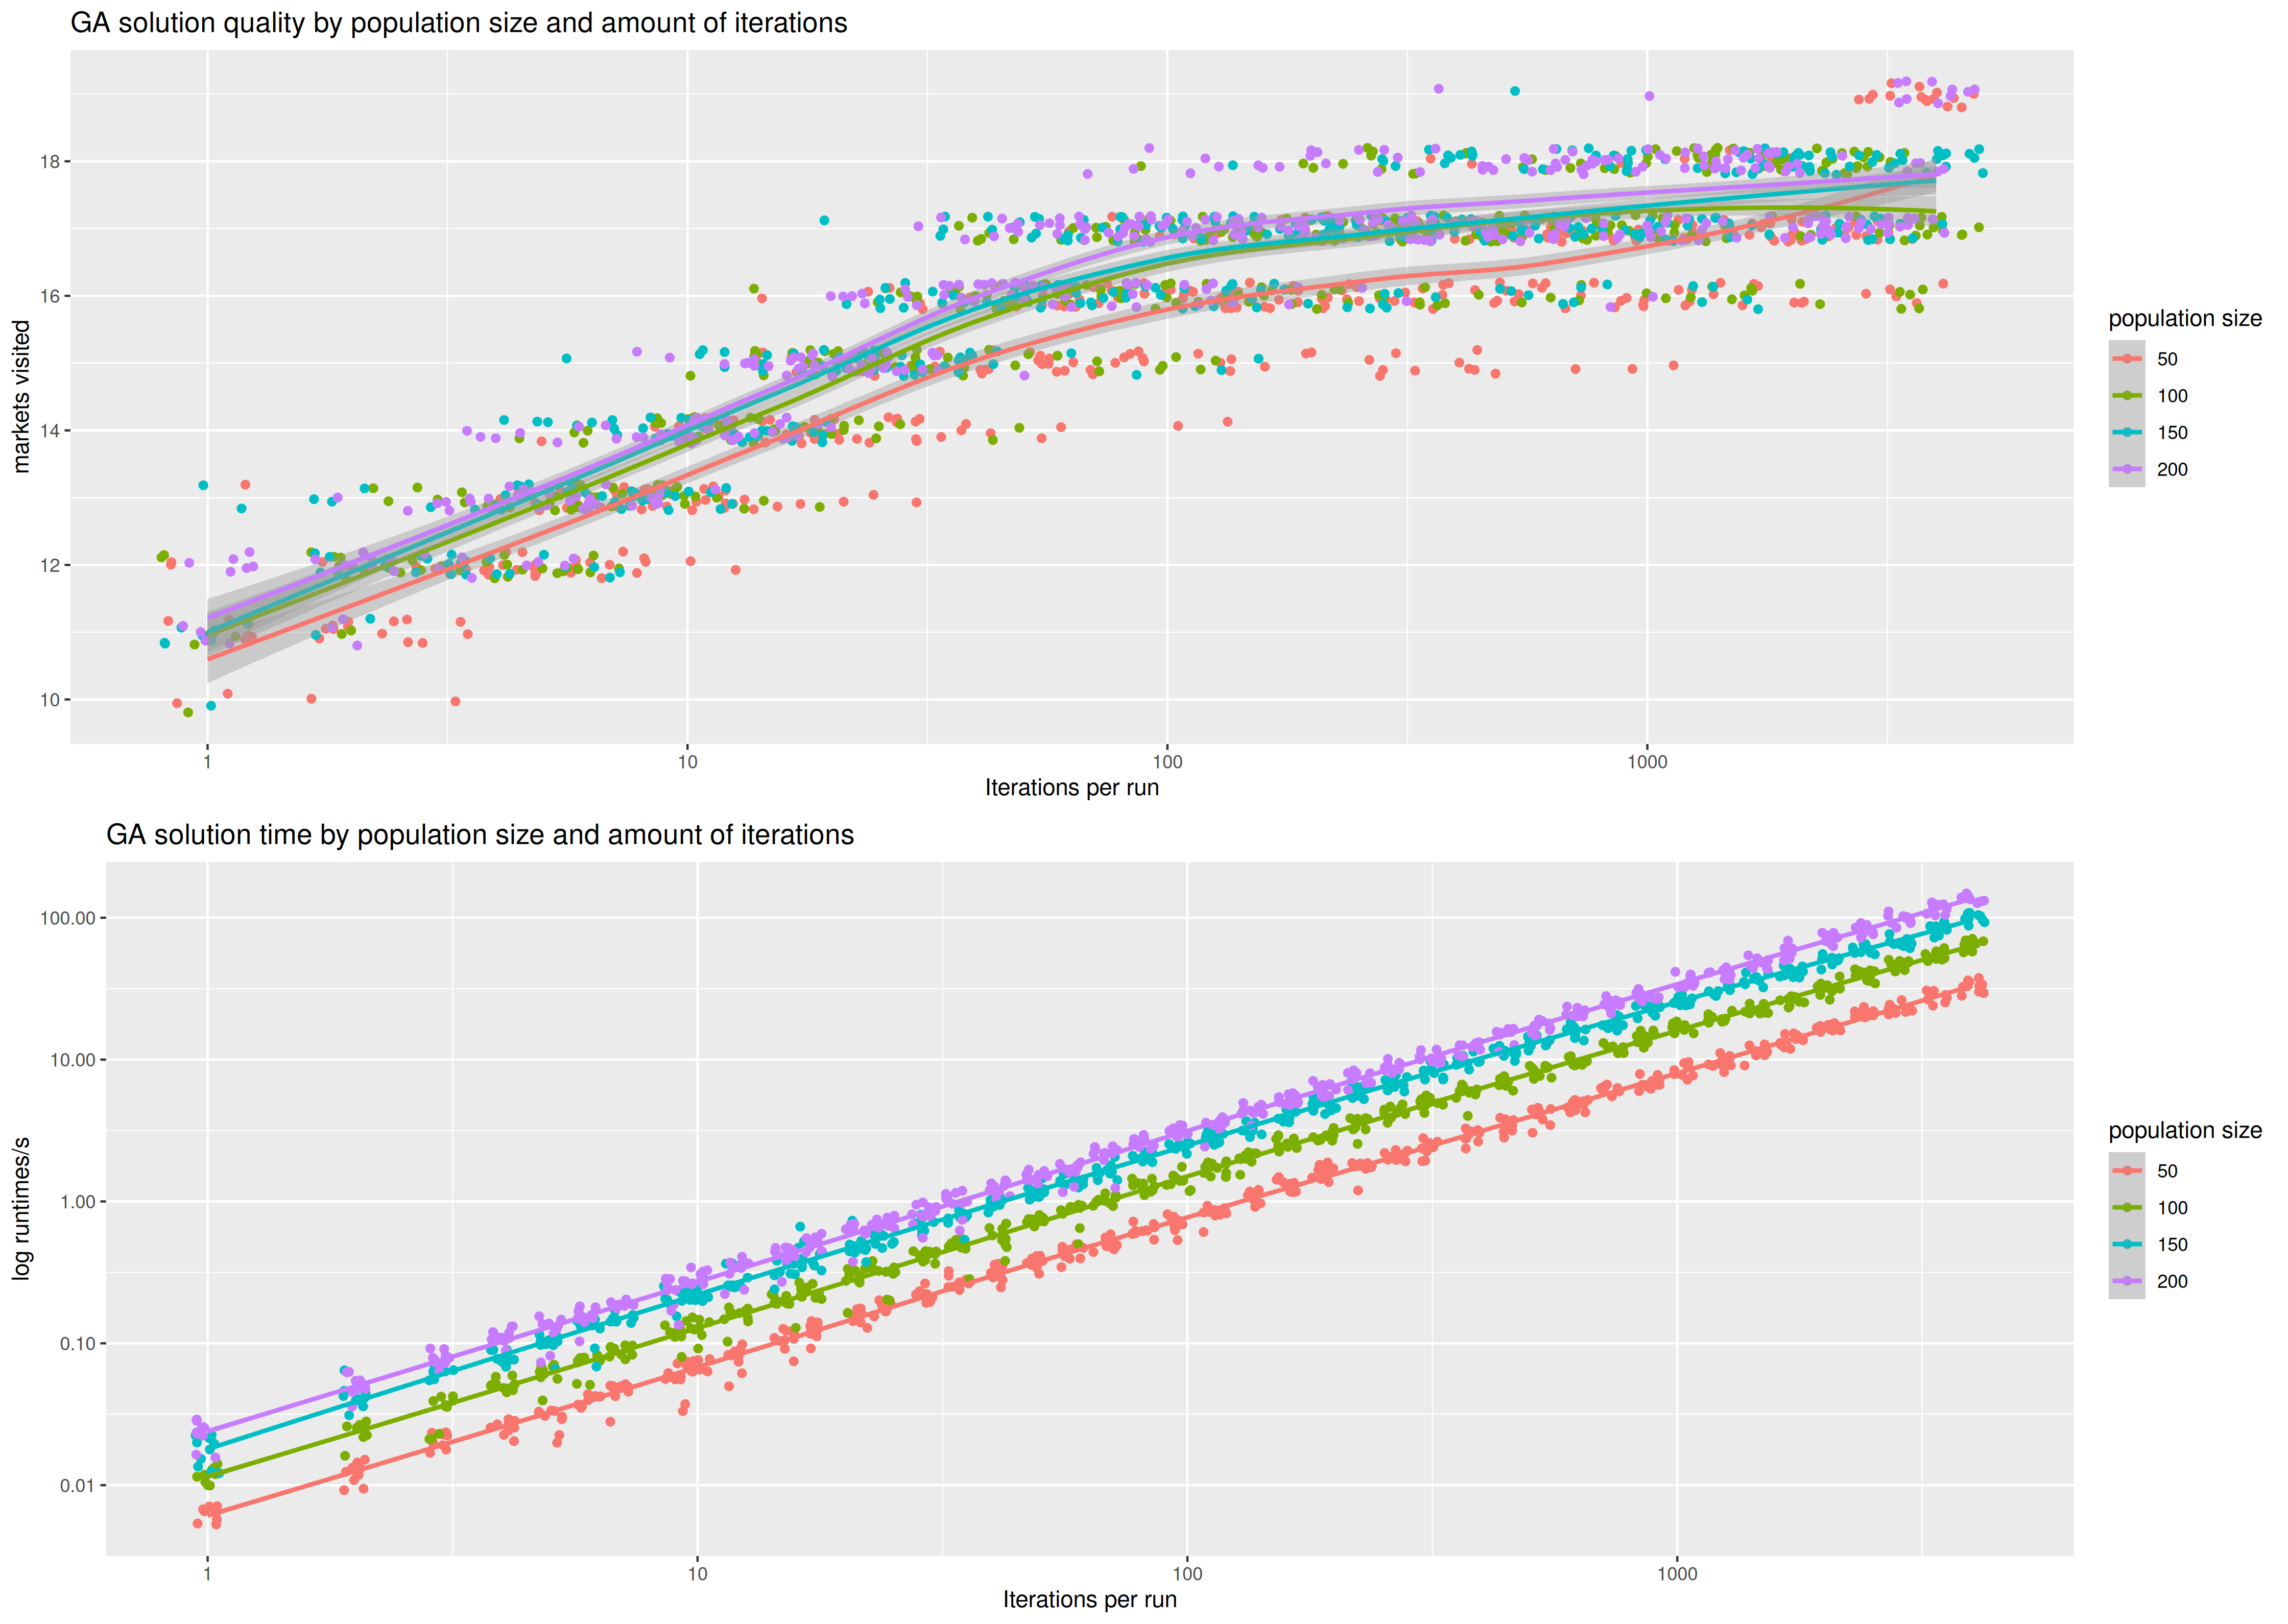
\includegraphics[width=\textwidth]{figures/tcmt_default_ggplot.png}
    \caption{Results for the original TCMT Instance for different population sizes and iterations}
    \label{fig:default_results}
\end{figure}

\begin{figure}
    \centering
    \includegraphics[width=\textwidth]{figures/Screenshot_20221127_195719.png}
    \caption{One Example of the best found route with nearly 19 full stops. The interactive version can be found 
\href{https://www.google.com/maps/dir/'48.1849955,16.3883483'/'48.1914751,16.3809322'/Stephansplatz,+1010+Wien/'48.2046241,16.3703338'/'48.2071865,16.3652063'/'48.2110893,16.3668794'/'48.2113909,16.3648319'/'48.2113909,16.3648319'/'48.207941,16.366853'/'48.197676,16.3696919'/'48.203354,16.3533211'/'48.2105267,16.3590678'/'48.2050248,16.3582693'/'48.199234,16.3483456'/'48.1954759,16.3360935'/'48.1993311,16.3177638'/'48.2128557,16.32487'/'48.2161089,16.3507476'/'48.202999,16.3595479'/@48.1991069,16.3461862,14.29z/data=!3m1!5s0x476d077ce3e5331d:0x75f9613b681cc472!4m116!4m115!1m5!1m1!1s0x0:0x589ca1fc5bea6c3b!2m2!1d16.3877346!2d48.1851373!1m5!1m1!1s0x0:0xb061cc711ea941ed!2m2!1d16.3809322!2d48.1914751!1m5!1m1!1s0x476d079f3e69c281:0x20563c156aa1fde!2m2!1d16.3734791!2d48.2088364!1m5!1m1!1s0x0:0x7d51d9cddf1ac199!2m2!1d16.3703907!2d48.204525!1m5!1m1!1s0x0:0x63d740da6abac406!2m2!1d16.3654971!2d48.2072951!1m5!1m1!1s0x0:0x81d571a836ccaa1!2m2!1d16.3671012!2d48.21108!1m5!1m1!1s0x0:0xe45c1f15ab2c2b5b!2m2!1d16.365302!2d48.2111478!1m5!1m1!1s0x0:0xe45c1f15ab2c2b5b!2m2!1d16.365302!2d48.2111478!1m5!1m1!1s0x0:0x78e5eb30a5c38527!2m2!1d16.3665236!2d48.2079776!1m5!1m1!1s0x0:0x5cbaec32a3408a2d!2m2!1d16.3696514!2d48.197609!1m5!1m1!1s0x0:0x5bfd3c40070cc712!2m2!1d16.3533211!2d48.203354!1m5!1m1!1s0x0:0x64d61847234d7df9!2m2!1d16.3590678!2d48.2105267!1m5!1m1!1s0x0:0xcee724536b265c36!2m2!1d16.3582693!2d48.2050248!1m5!1m1!1s0x0:0x7f4e28fc3fc94fa3!2m2!1d16.3483456!2d48.199234!1m5!1m1!1s0x0:0xc900d475e5dff5aa!2m2!1d16.3360935!2d48.1954759!1m5!1m1!1s0x0:0xa677fdf4c5ad2193!2m2!1d16.3177638!2d48.1993311!1m5!1m1!1s0x0:0x64e98061b63aeda5!2m2!1d16.32487!2d48.2128557!1m5!1m1!1s0x0:0xc6509becb69403f7!2m2!1d16.3507476!2d48.2161089!1m5!1m1!1s0x0:0x3f59d4e806788e43!2m2!1d16.3595479!2d48.202999!3e2}{here}}
    \label{fig:optimal_route}
\end{figure}


\begin{figure}
    \centering
    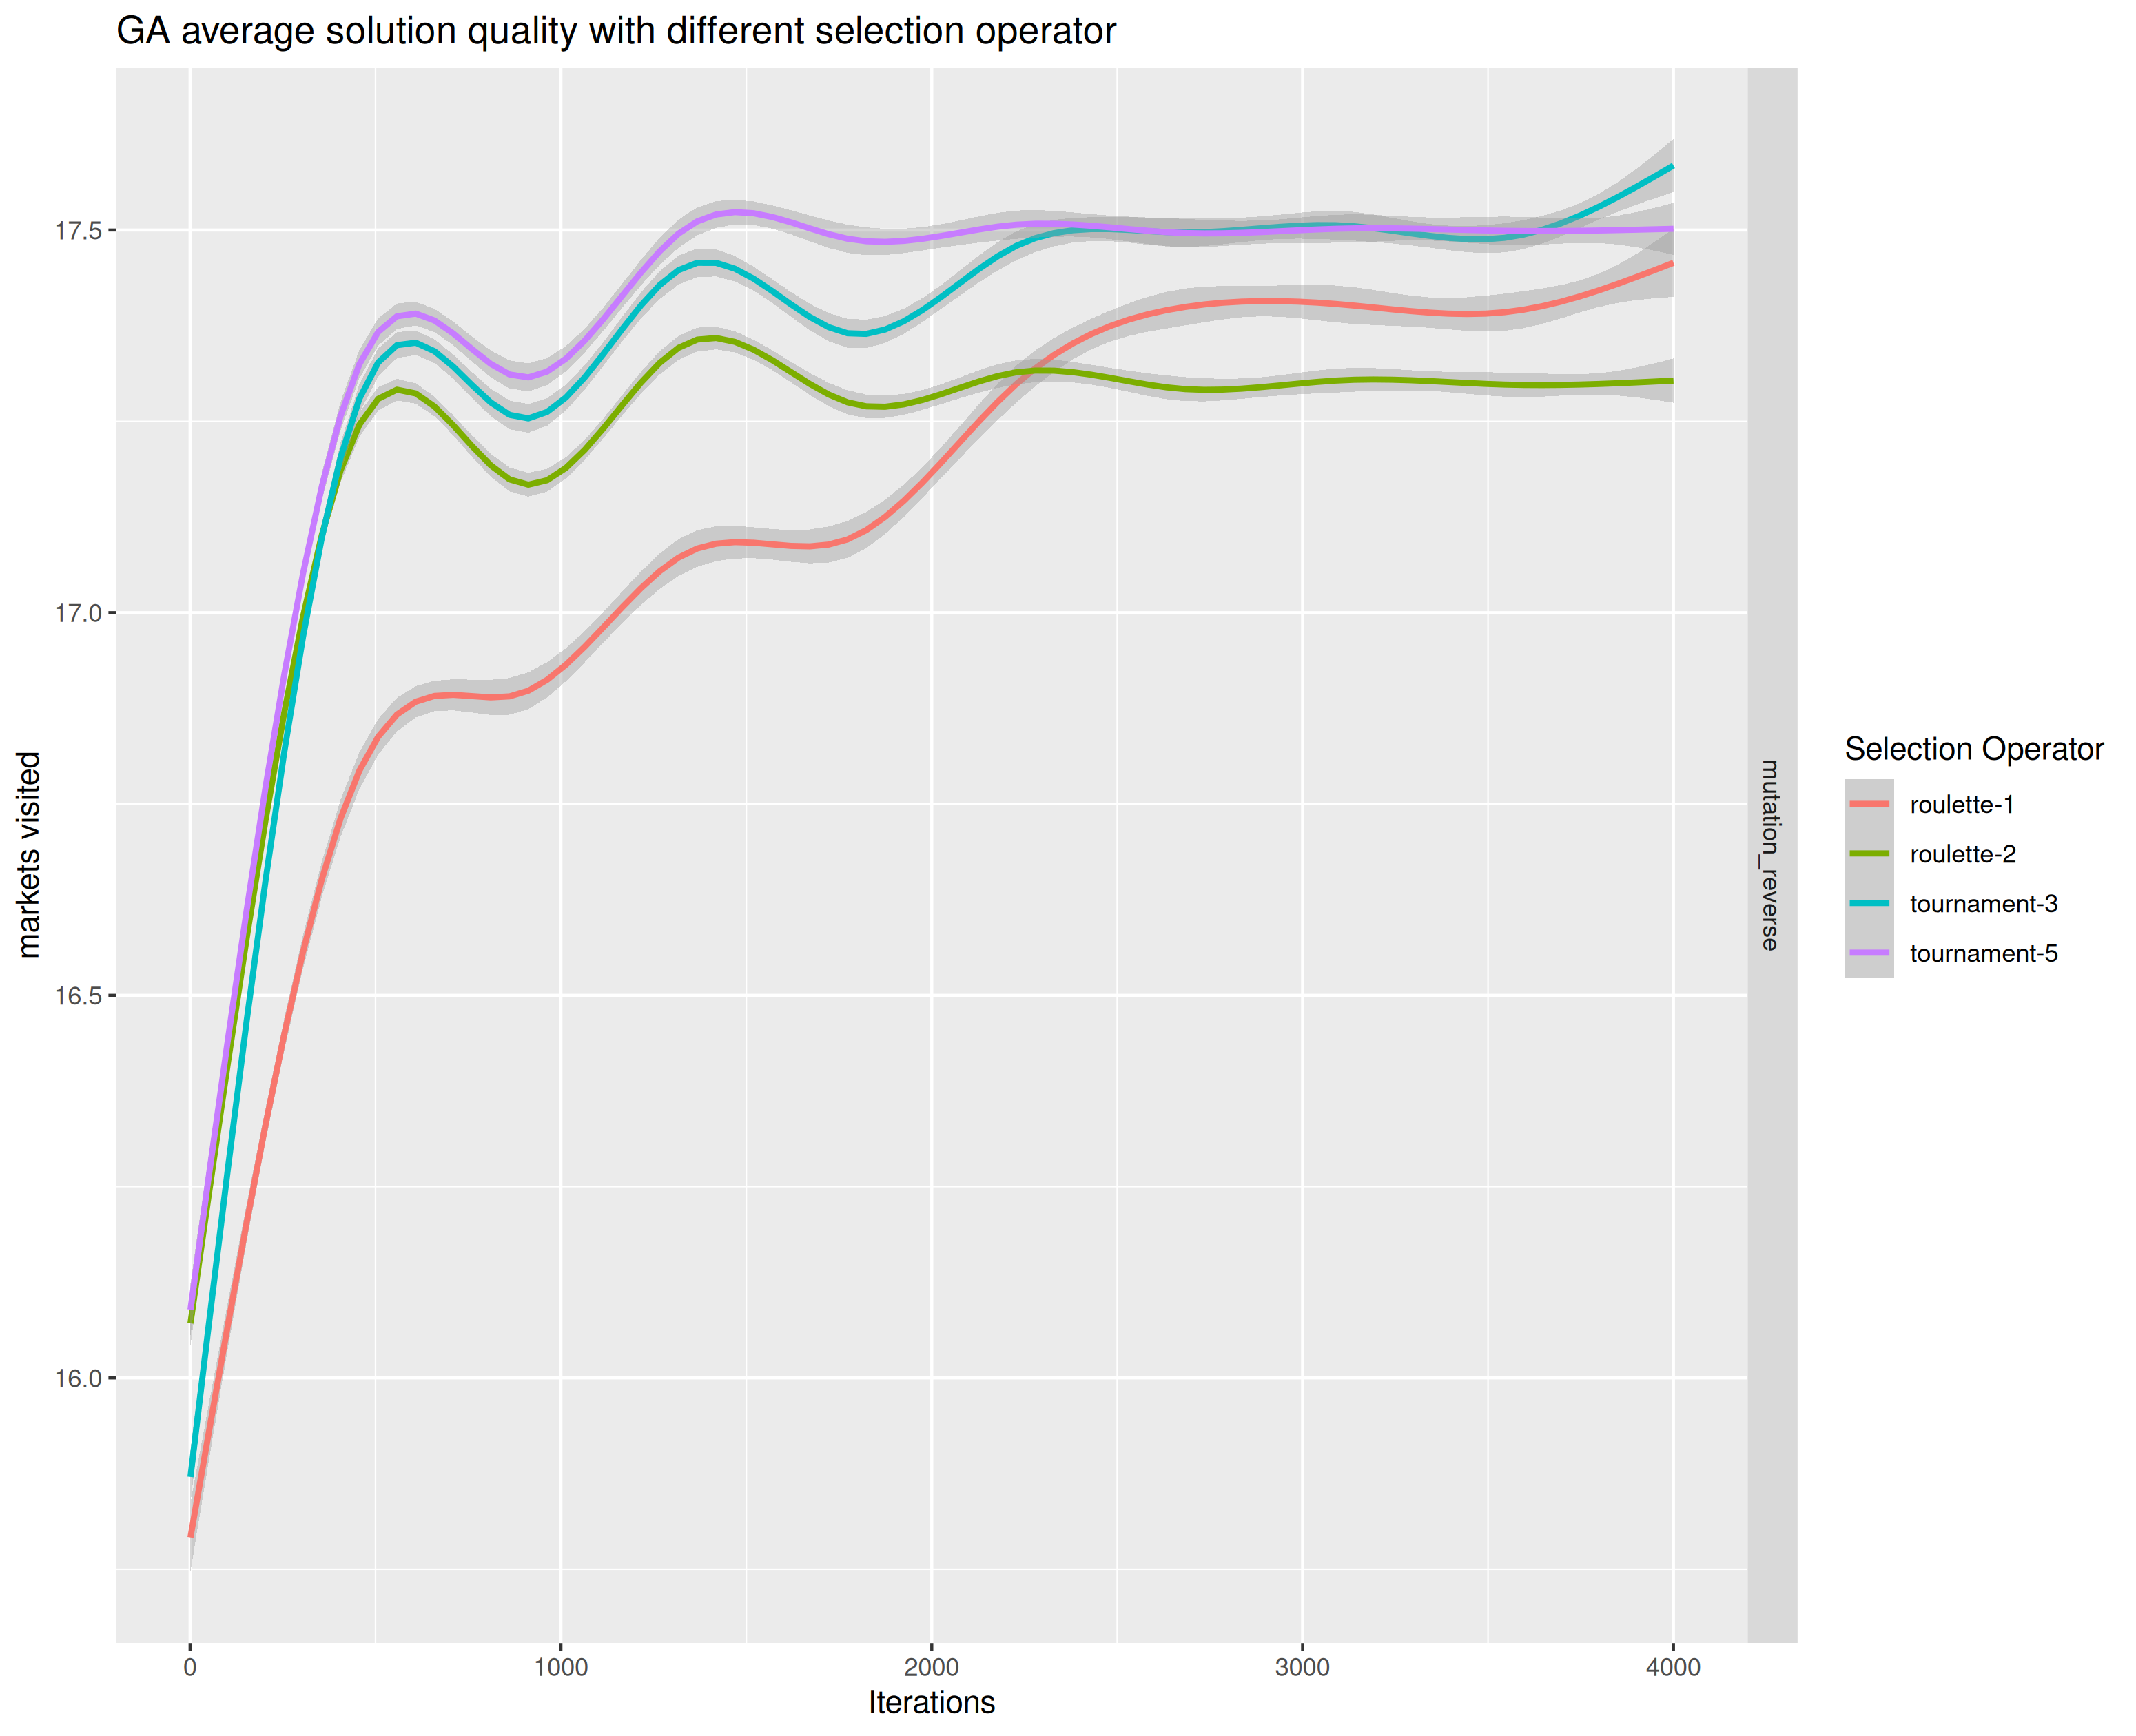
\includegraphics[width=0.75\textwidth]{figures/runs3_ggplot.png}
    \caption{Experiment for comparing different selection operators. Tournament selection performs best.}
    \label{fig:selection}
\end{figure}

\begin{figure}
    \centering
    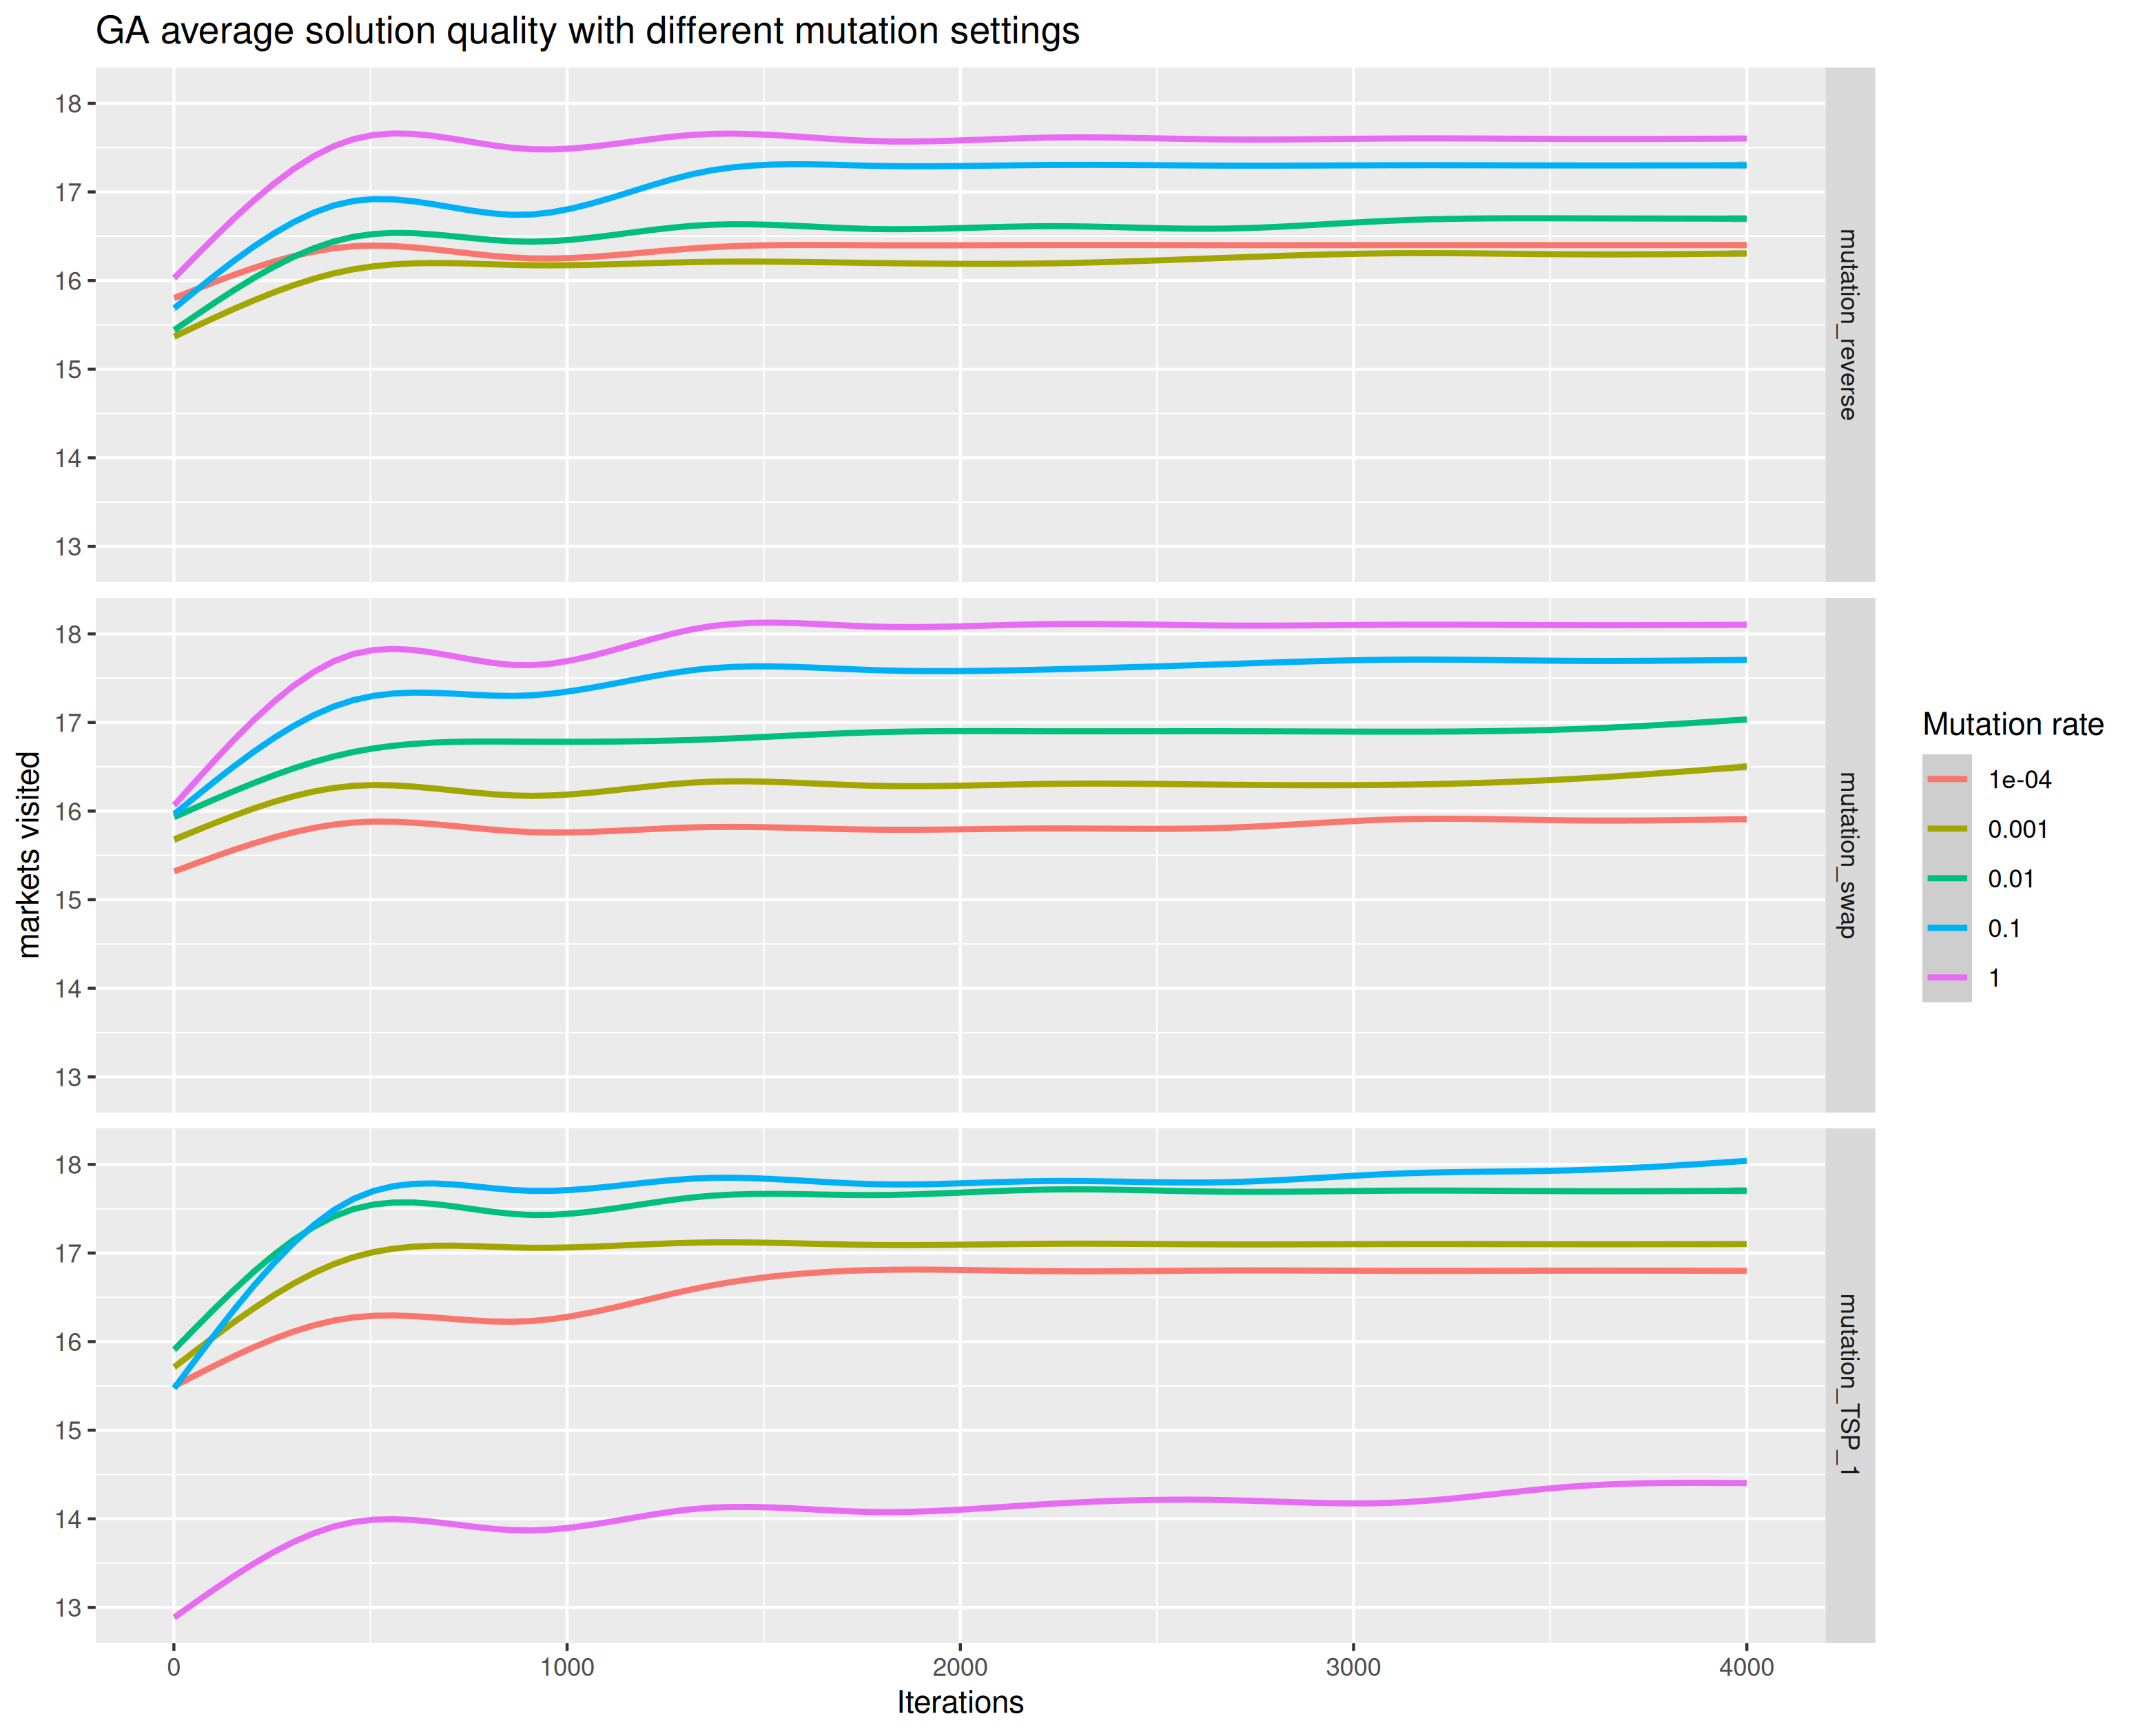
\includegraphics[width=0.75\textwidth]{figures/runs2_ggplot.png}
    \caption{Experiment for comparing different mutation settings. Swap Mutation shows better expected results than reversing mutation. TSP-Mutation showed good results with smaller learning rates.}
    \label{fig:mutation}
\end{figure}


% \href{https://www.google.com/maps/dir/'48.1849955,16.3883483'/'48.1914751,16.3809322'/Stephansplatz,+1010+Wien/'48.2046241,16.3703338'/'48.2071865,16.3652063'/'48.2110893,16.3668794'/'48.2113909,16.3648319'/'48.2113909,16.3648319'/'48.207941,16.366853'/'48.197676,16.3696919'/'48.203354,16.3533211'/'48.2105267,16.3590678'/'48.2050248,16.3582693'/'48.199234,16.3483456'/'48.1954759,16.3360935'/'48.1993311,16.3177638'/'48.2128557,16.32487'/'48.2161089,16.3507476'/'48.202999,16.3595479'/@48.1991069,16.3461862,14.29z/data=!3m1!5s0x476d077ce3e5331d:0x75f9613b681cc472!4m116!4m115!1m5!1m1!1s0x0:0x589ca1fc5bea6c3b!2m2!1d16.3877346!2d48.1851373!1m5!1m1!1s0x0:0xb061cc711ea941ed!2m2!1d16.3809322!2d48.1914751!1m5!1m1!1s0x476d079f3e69c281:0x20563c156aa1fde!2m2!1d16.3734791!2d48.2088364!1m5!1m1!1s0x0:0x7d51d9cddf1ac199!2m2!1d16.3703907!2d48.204525!1m5!1m1!1s0x0:0x63d740da6abac406!2m2!1d16.3654971!2d48.2072951!1m5!1m1!1s0x0:0x81d571a836ccaa1!2m2!1d16.3671012!2d48.21108!1m5!1m1!1s0x0:0xe45c1f15ab2c2b5b!2m2!1d16.365302!2d48.2111478!1m5!1m1!1s0x0:0xe45c1f15ab2c2b5b!2m2!1d16.365302!2d48.2111478!1m5!1m1!1s0x0:0x78e5eb30a5c38527!2m2!1d16.3665236!2d48.2079776!1m5!1m1!1s0x0:0x5cbaec32a3408a2d!2m2!1d16.3696514!2d48.197609!1m5!1m1!1s0x0:0x5bfd3c40070cc712!2m2!1d16.3533211!2d48.203354!1m5!1m1!1s0x0:0x64d61847234d7df9!2m2!1d16.3590678!2d48.2105267!1m5!1m1!1s0x0:0xcee724536b265c36!2m2!1d16.3582693!2d48.2050248!1m5!1m1!1s0x0:0x7f4e28fc3fc94fa3!2m2!1d16.3483456!2d48.199234!1m5!1m1!1s0x0:0xc900d475e5dff5aa!2m2!1d16.3360935!2d48.1954759!1m5!1m1!1s0x0:0xa677fdf4c5ad2193!2m2!1d16.3177638!2d48.1993311!1m5!1m1!1s0x0:0x64e98061b63aeda5!2m2!1d16.32487!2d48.2128557!1m5!1m1!1s0x0:0xc6509becb69403f7!2m2!1d16.3507476!2d48.2161089!1m5!1m1!1s0x0:0x3f59d4e806788e43!2m2!1d16.3595479!2d48.202999!3e2}{Example for an optimal route pasted back into google Maps}


\section{Discussion}

In conclusion the chosen approach via genetic algorithms seemed to work well.
While gauging performance with only one approach and without any optimal results for the instances is not that trivial, the original instance could be used to produce solutions of up to 19 visited Christmas markets, where the last one is not visited for the full 30 minutes.
This route, also depicted in figure \ref{fig:optimal_route} is included in a text file in the submission package.

While some experiments with different operators have been made, proper gridsearch over the amount of hyper-parameters possible takes a long time and there are many ways to further tweak the performance of the algorithm.

The default settings for the hyperparameters preselected for the TSP proved fine for this specific problem as well.

One of the important lessons learned was not to blindly apply operators which are pre-implemented, as especially for this representation, the wrong crossover or mutation operator easily breaks the result.


% Lessions learned, how well did it work

% Seems to have worked quite well, the TSP implementation did most of the work and the target function was enough to make it work.

% Gridsearch over hyperparameters might be a good idea to see effect of differently tuned parameters.

% Experiment setup was costly though, and there are many things to tweak (selection of operators, at least one hyperparameter per operator...).

% Hence the selection of operators was kept, as it is most likely tuned for good performance for general TSP(-like) Problems. 


\end{document}